\documentclass[11pt, a4paper]{scrartcl}
\usepackage[affil-it]{authblk} 
\usepackage{etoolbox}
\usepackage{lmodern}
\usepackage[sort]{natbib}      % references
\usepackage[nottoc]{tocbibind} % bib om toc
\usepackage{hyperref}          % clickable links
\usepackage[all]{hypcap}       % for going to the top of an image when a figure reference is clicked
\usepackage{cleveref}
\usepackage{graphicx}
\usepackage{rotating}
\graphicspath{ {img/} }

\makeatletter
\patchcmd{\@maketitle}{\LARGE \@title}{\fontsize{16}{19.2}\selectfont\@title}{}{}
\makeatother

\renewcommand\Authfont{\fontsize{14}{14.4}\selectfont}
\renewcommand\Affilfont{\fontsize{12}{10.8}\itshape}

\setlength\parindent{0pt}
\setlength{\parskip}{1em}

\bibliographystyle{humannat}

\title{An Infrastructure to Store and Analyse Seismic Data as Suffix Trees}
\subtitle{A dissertation submitted in partial fulfilment of the requirements for the MSc in Data Analytics}
\author{Thomas Taylor}
\affil{Department of Computer Science and Information Systems, Birkbeck College, University of London}
\date{September 2016}

\begin{document}
	\pagenumbering{roman}
	\maketitle
	\begin{itshape}
		This report is substantially the result of my own work except where explicitly indicated in the text. I give my permission for it to be submitted to the JISC Plagiarism Detection Service. I have read and understood the sections on plagiarism in the programme Handbook and the College website.
		
		The report may be freely copied and distributed provided the source is explicitly acknowledged.
	\end{itshape}
	\newpage
	
	\section*{Abstract}
	The purpose of this project is to develop an infrastructure and tool set for converting raw seismic time series data into a searchable string using SAX (\textbf{S}ymbolic \textbf{A}ggregate appro\textbf{X}imation) and then to store this data as a suffix tree for fast searching and analysis.  An interface will then be developed to enable the searching of these suffix trees and provide visualisation of the data.  This will enable the searching for similar patterns over time or between stations after an event.
	
	Potential applications of the software could be:
	\begin{itemize}
		\item Automatically finding the arrival times of events
		\item Correlating events across multiple stations
		\item Finding similar events at a given location at other times
	\end{itemize}
	
	The code should ideally be re-usable where possible in a project to receive live streaming data from many stations.
	\newpage
	\tableofcontents
	\thispagestyle{empty}
	\cleardoubleemptypage
	\pagenumbering{arabic}
		
	\section{Background}
	\subsection{Seismic Waves}
	\label{sec:seismicwaves}
	Seismic waves take on two main forms, body waves and surface waves.  Body waves are those that travel through the interior of the earth and are the fastest travelling.  The body waves are comprised of \textbf{P} (primary) waves which are compressional waves, travel fastest and thus arrive first.  \textbf{S} (secondary) waves are shear waves and travel more slowly, thus arrive later.  The separation between the phases is related to the distance of the earthquake and the local velocity structure. The surface waves travel only along the earth's crust and, as they are confined to shallow depths where seismic velocities are slow, will normally arrive much later than the body waves.
	
	A seismic station records movement over three axis: vertical (\textbf{z}) alongside horizontal in terms of north-south (\textbf{n}) and east-west (\textbf{e}).  Due to seismic velocities generally increasing with depth, P waves arrive at a seismic station close to the vertical axis.  As a result, P waves can be measured as a simple metric of displacement along the Z axis.  S waves follow similar ray paths, but have their particle motion perpendicular to the direction of propagation.  As a result, they manifest on a seismogram as movement on both the n and e axis. The geometry of the fault tends to have a bearing on the orientation of the displacement so the two horizontal axis of movement cannot be easily combined in to a single metric for time series analysis.
	
	\subsection{Symbolic Aggregate Approximation (SAX)}
	SAX (\textbf{S}ymbolic \textbf{A}ggregate appro\textbf{X}imation) \citep{sax} is a technique where by a single dimension of a time series is reduced to a string of symbols for pattern matching.  The technique involves first transforming the normalised time-series in to a Piecewise Aggregate Approximation (\textbf{PAA}) which is then represented by a fixed number of symbols.
	
	For the PAA, the data is first divided into equal sized time frames (see diagram below), then the mean deviation from zero of each frame is calculated.  An appropriate number of breakpoints symmetrical along the x-axis are created so that they follow a Gaussian distribution and a symbol assigned to each range between the breakpoints.  Then for each frame, a symbol is assigned based on which range the mean falls in to.  The symbols assigned to each frame are then concatenated in to a string and it is this string that gives the SAX representation of that data.  The width of the time frame and the number of discrete regions would be two parameters passed to this process alongside the data.
	\begin{figure}[h]
		\centering
		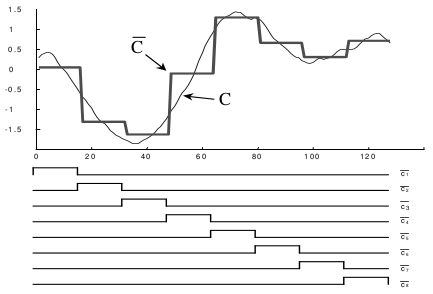
\includegraphics[scale=0.5]{paa.png}
		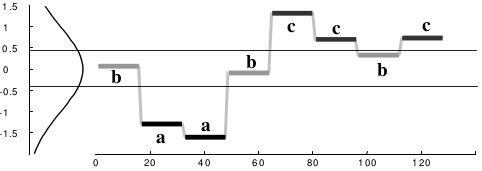
\includegraphics[scale=0.5]{sax.png}
		\caption{Diagrams showing PAA to SAX on a time-series (taken from \cite{sax})}
	\end{figure}
	
	\subsection{Suffix Trees and the related infrastructure at Birkbeck}
	Suffix trees \citep{suffix} are a representation of a string designed for performing search related algorithms.  They are based on a suffix trie of a given string \textbf{T}.  The trie is constructed using all of the suffixes of \textbf{T} with a terminator character not used in the alphabet appended to the end of \textbf{T}.  The terminator is deemed to be lexicographically of lower priority than all of the other characters to ensure that a prefix of a string would appear before that string (such as in \textit{as} before \textit{ash}).  In the following example, the suffixes of \textit{T: abaaba} would produce the following suffixes with \textbf{\$} applied as a terminator.
	\begin{figure}[h]
		\centering
		\includegraphics[scale=0.5]{suffix_trie.png}
		\caption{Example Suffix Trie}
	\end{figure}
	
	This allows for efficient searching and counting substrings of \textbf{T} by following the trie from the root node.  Each substring \textbf{S} of \textbf{T} is a prefix of a path starting at the root.  It allows for counting occurrences of the substring by finding the number of leaf nodes that can be reached from the end of the substring.  This format is not particularly space efficient as it has an upper bound storage in the order of \textit{$O(n^{2})$}.
	
	A far more efficient way to store and query the trie is to store it as Suffix Trees.  In order to produce a suffix tree from a trie, the non-branching nodes are firstly reduced (or coalesced) in to a single edge.  The original string \textbf{T} is then stored along side the tree and the labels further reduced to a starting position and offset within \textbf{T}.  The leaf nodes become labels to the offset of the suffix in the string.  This reduces the upper bound storage to \textit{$O(n)$} and results in a tree for our example \textbf{T} as seen in \cref{fig:tree}.
	\begin{figure}[h]
		\label{fig:tree}
		\centering
		\includegraphics[scale=0.5]{suffix_tree.png}
		\caption{Example Suffix Tree (edges shown as text and as positions/offsets)}
	\end{figure}
	
	This technique of building the tree is considered naive though as it is again very inefficient (being computationally in the order of \textit{$O(n^{3})$}).  It is far more desirable to achieve time-linear \textit{O(n)} construction of the tree.  An example of this is the Ukkonens Algorithm \citep{ukkonens}.  The algorithm is too long for inclusion but effectively starts with the implicit suffix tree of a string of length 1 and conditionally extends the tree on each iteration of adding a character.
	
	At Birkbeck, an infrastructure has been developed to load and query Suffix Trees \citep{bbk-suffix}.  At a high level it is based on language models but should be extendable to time series by the use of SAX.  There is current work in progress to utilise external memory (in this case Solid State Drives) to back the loaded Suffix Trees.  This would massively increase the maximum size of a tree to be queryable.  The current libraries to utilise this are written in Python however there is currently a refactor happening to C due to Python not being particularly computationally efficient because of its interpreted nature.  The trees in this implementation are stored as k-truncated trees for practical reasons.
	
	\section{Program Architecture}
	\subsection{Overview}
	It was a stipulation that the project be completed (where possible) using Python.  Specifically Python 3 was selected as Python 2 has been marked approaching end-of-life.
	
	The project was broken down in to five discreet components.  A User Interface, a graph renderer to generate the graphs, a service to perform PAA and SAX analysis on the raw data, an API for the time-series database and a service to interface with the existing suffix tree infrastructure.
	
	\begin{figure}[h]
		\centering
		\includegraphics[scale=0.5]{Architecture.png}
		\caption{Architecture of the Project}
	\end{figure}
	
	\subsubsection{Interface}
	It was decided to make the user interface web based to avoid having to build software for different platforms and reduce dependency on the end-users device.
	
	The interface supports importing and browsing of data, rendering of plots of both raw data and data with PAA and SAX applied and the loading of data in to a suffix tree.
	
	\subsubsection{Graph Renderer}
	This service reads from either the TSDB API directly (for plots of raw data) or via the PAA/SAX service for plots to show how the SAX data was created.
	
	\subsubsection{PAA/SAX}
	This is a stateless service that reads data from the TSDB API and performs parameterised PAA and SAX returning the data for consumption either by the graph renderer or the Suffix Tree Store.
	
	\subsubsection{TSDB API}
	An API was written to standardise the getting and putting of data to and from the time-series database.  This was designed to allow the changing of the underlying datastore to databases with differing APIs without having to alter the other components.
	
	\subsubsection{Suffix Tree Store}
	
	\subsection{Micro-services}
	A decision was taken early on in the project to break the various aspects of it in to smaller services each exposed by an HTTP API.  This methodology reduces the potential impact of modifications on a component (or even a complete refactor of said component) on another so long as the API is maintained.  It also allows for more CPU or IO intensive parts of the application to be distributed on different physical nodes to avoid bottlenecks in performance.
	
	\subsection{Docker}
	Docker is an open source project that allows a single (or a small number) of processes to act in an isolated namespace (a.k.a a container) on a Linux based OS.  By defining a manifest (a Dockerfile), the commands required to build and run a component of the project from scratch can be documented and executed in a repeatable way.  By using Docker Compose, the individual services could be linked together in such a way that the whole project could be started on a single machine or farmed out to a cluster such as docker Swarm or Amazon ECS.
	
	This provides two main benefits, firstly as each container is regularly rebuilt in an automated way, it is known that all steps to bootstrap any component are complete.  Secondly it ensures that the whole project is portable, acting the same in a development environment as in a production ready deployment.
	
	\subsection{Frameworks}
	CherryPy was selected as the Python web framework to define the APIs.  It allows for API construction by use of mounting python classes in a tree and then methods to be exposed by use of a built-in decorator.  It also natively supports JSON and the Jinja2 templating language used by the interface.
	
	The interface was written using a minimalist implementation of the HTML/CSS/Javascript framework Bootstrap.  Bootstrap provides a clean skeleton to write an HTML interface without having to worry about different browsers and platforms rendering the interface differently.
	
	\subsection{Time-series Database}
	It was important to select a database specifically designed for querying time-series data due to the range style queries and large number of datapoints to be analysed.  During the course of development, three time-series databases were tested for implementation.  Namely Graphite, InfluxDB and OpenTSDB.
	
	Graphite would have been the simplest to implement as its storage engine is small and lightweight (and also written in Python) and it stores the data in a relatively easy to use format (RRD) in local flat files.  Also the API to graphite is extremely simple to implement. Unfortunately it did not support sub-second time resolution and was not trivial to patch.
	
	InfluxDB is a much newer entrant to the time-series database world, written in Golang and targeted at an enterprise market for gathering metrics across a large distributed infrastructure.  A basic driver for this database was written and early tests seemed positive.  However during large data imports and over large ranging queries, its memory usage ballooned out of control often being killed by the OOM (Out Of Memory) process killer on the development workstation with 32GiB of RAM.  In addition, the authors of the project appeared to be moving away from a fully featured Open Source product by making features premium only (such as the ability to do clustering).  As such, it was deemed unsuitable.
	
	The final time-series database to be considered was OpenTSDB.  Unlike the first two options, OpenTSDB is not a self standing product.  It relies on HBase (and in turn HDFS) from the Apache Hadoop project to run.  As such, for production or long running use, multiple nodes are required to have an effective and performant system.
	
	It does however support sub-second time resolution and has a well documented HTTP API.  It also supports a development mode not requiring a full Hadoop infrastructure to run and in this mode, has the ability to run in a docker container.
	\bibliography{bibliography}
	
\end{document}